\documentclass[12pt,conference,compsocconf]{../IEEEtran}
\usepackage{xltxtra}
%\usepackage{subfig}
%\usepackage{booktabs}
\usepackage{flushend}
\usepackage[numbers,sort&compress]{natbib}
\setmainfont{Times New Roman}

\begin{document}

\title{Chemical-Genetic Profiling and Its Applications}
\author
{
\IEEEauthorblockN
{
Hongjian Li
\IEEEauthorblockA
{
Department of Computer Science and Engineering\\
Chinese University of Hong Kong\\
hiji@cse.cuhk.edu.hk
}
}
}
\maketitle

\begin{abstract}

Chemical-genetic profiling of bioactive compounds has been repeatedly proved to be a powerful tool for identifying novel drugs, mode of actions of drugs and drug targets, and for better understanding the relation between genotype and phenotype. In the past two decades, research mainly concentrated on applying chemical-genetic profiling to the yeast genome, but seldom investigated into higher organisms like mammals, or higher level of practical applications like drug synergy. This survey briefly reviews the popular experimental techniques and computational methods for constructing and analyzing chemical-genetic profiles and discusses their pros and cons. In the foreseeable future, as both the number of bioactive compounds and the number of sequenced genes increase, more and more chemical-genetic profiles will emerge. How to establish an universal database to accommodate diverse output from various research groups, and how to correctly and properly utilize such ressources for better drug discovery will become challenging issues.

\end{abstract}

%\begin{IEEEkeywords}

%Chemical-Genetic Profiling, Drug-Target Pathway, Mode-of-Action

%\end{IEEEkeywords}

\section{Introduction}

Chemical genetics refers to the study of genetic responses to chemical compounds. In genome-wide level, it is called chemical genomics or chemogenomics. It embraces multiple early phase drug discovery technologies ranging from target identification and validation, through compound design and chemical synthesis, to biological testing and ADME profiling.

Chemical-genetic profiling is nowadays gaining more and more importance and popularity as it provides a valuable tool for a wide variety of biological applications, including but not limited to rapid identifications of novel drugs, mode of actions (MOAs) of drugs and drug targets, and understanding biological systems to a better extend by relating genotype and phenotype.

\section{Motivation}

Partly due to the massive failure of antimicrobial target-based \textit{in vitro} screening strategies over the past 20 years, chemical-genetic profiling is preferred over high-throughput screening in certain applications thanks to its ability to rapidly characterize compounds in an unbiased fashion and provide rich, functional information to elucidate their MOAs and targets.

High-throughput screening is mainly limited by two factors. The pharmaceutical targets are usually limited to a small subset of specific proteins, and it could be very difficult to conduct a comprehensive screening given the facts that the small molecule chemical space consists of as many as 10\textsuperscript{60} chemical compounds and the rate of compound synthesis via combinational chemistry is constantly increasing. In contrast, chemical-genetic profiling can be genome-wide and even interspecies.

\section{Background}

Chemical-genetic profiling basically measures the quantitative values of growth defects of deletion strains under exposure to chemicals. The foundation of chemical-geneitic approach was laid with the idea to sequence the 12.5-megabase yeast genome in the 1980s. Figure \ref{fig:1081-1} shows the six major steps for yeast fitness profiling of pooled deletion strains. Experimental detail can be found in the original publicaton \citep{1081}.

\begin{figure}
\centering
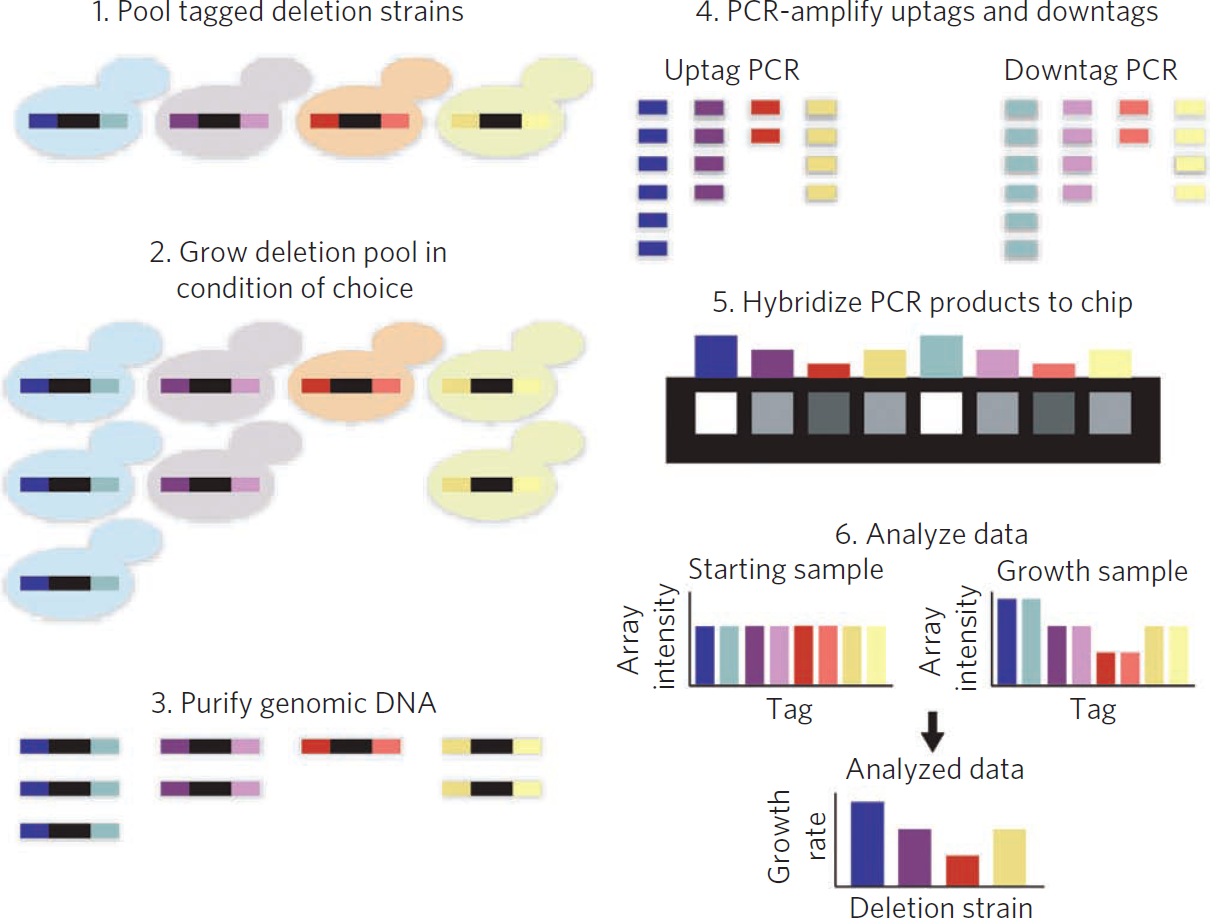
\includegraphics[width=\linewidth]{1081-1.png}
\caption{Yeast fitness profiling of pooled deletion strains. Figure reprinted from \citep{1081}.}
\label{fig:1081-1}
\end{figure}

Figure \ref{fig:1082-1} compares genetic, chemical-genetic, and chemical-chemical profiling. In the case of chemical-genetic profiling, one gene product is inactivated via gene deletion and the other is inactivated by chemical inhibition (Figure \ref{fig:1082-1}a). Red indicates a significant drug-gene interaction (Figure \ref{fig:1082-1}b). Such quantative values can be used to predict the target process of unknown agents. In the case of chemical-genetic profiling, known compounds on the X-axis are clustered based on known mode of action or function, and the Y-axis shows clustering of other unknown genes with similar profiles.

\begin{figure}
\centering
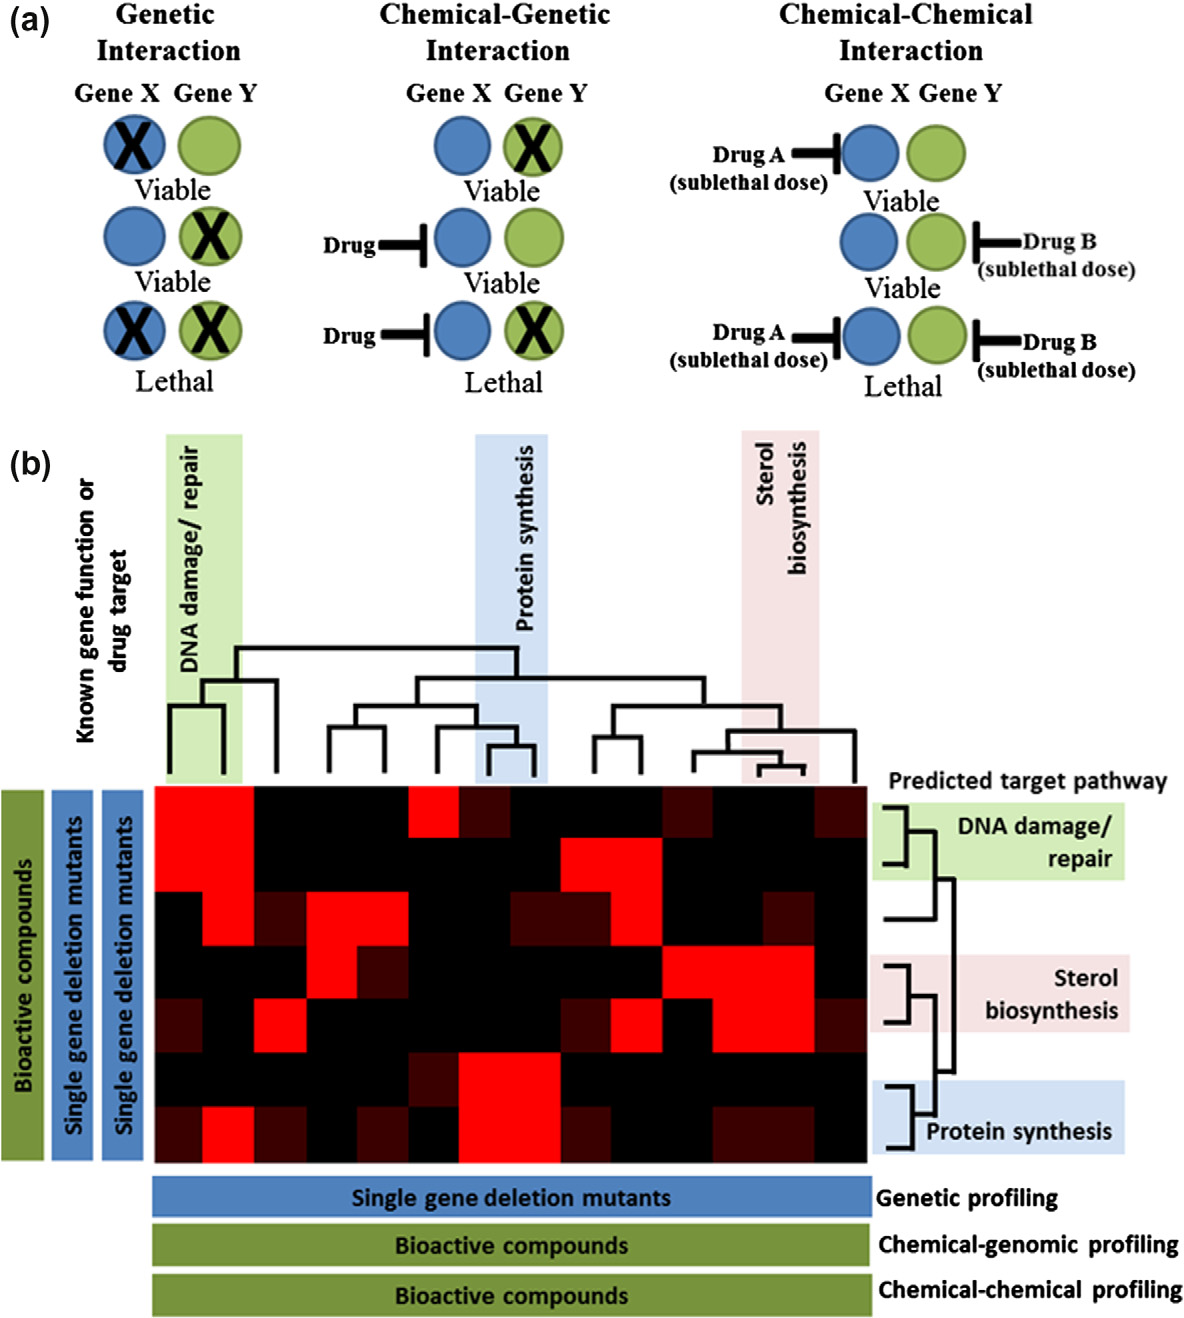
\includegraphics[width=\linewidth]{1082-1.png}
\caption{Comparison of genetic, chemical-genetic, and chemical-chemical profiling. Figure reprinted from \citep{1082}.}
\label{fig:1082-1}
\end{figure}

With the available data produced by chemical-genetic profiling, computational methods are then applied for in-depth analysis. Popular approaches include 2D hierarchical clustering, probabilistic sparse matrix factorization (PSMF) and bayesian factor model. 

\section{Compendium of Chemical-Genetic Interaction}

In \citeyear{1078}, \Citeauthor{1078} generated a compendium of chemical-genetic interaction profiles by testing the collection of viable yeast haploid deletion mutants for hypersensitivity to 82 compounds and natural product extracts. They then applied both a hierarchical clustering and a PSMF method, which allows a gene or compound to be associated with more than one group. Eventually they managed to  tamoxifen, a breast cancer therapeutic, was found to disrupt calcium homeostasis and phosphatidylserine (PS) was recognized as a target for papuamide B, a cytotoxic lipopeptide with anti-HIV activity. \citep{1078}

\section{Protein Complex-Based Bayesian Factor Model}

In \citeyear{1079}, \Citeauthor{1079} \citep{1079}.
\citep{1080}
\citep{1103} tutorial
\citep{1081} is state-of-the-art review.
\citep{1082} is state-of-the-art review.

Comparison
Have your own evaluation
Use others results and give reasons

\section{Discussion}

Summary on current works
  Avoid overlapping with existing reviews

\section{Prospectives}

What will be done in the future?
  Consequences of current breakthroughs
  Bottleneck in the whole picture

\bibliographystyle{unsrtnat}
\bibliography{../refworks}

\end{document}
